\documentclass{article}\usepackage[]{graphicx}\usepackage[]{xcolor}
% maxwidth is the original width if it is less than linewidth
% otherwise use linewidth (to make sure the graphics do not exceed the margin)
\makeatletter
\def\maxwidth{ %
  \ifdim\Gin@nat@width>\linewidth
    \linewidth
  \else
    \Gin@nat@width
  \fi
}
\makeatother

\definecolor{fgcolor}{rgb}{0.345, 0.345, 0.345}
\newcommand{\hlnum}[1]{\textcolor[rgb]{0.686,0.059,0.569}{#1}}%
\newcommand{\hlsng}[1]{\textcolor[rgb]{0.192,0.494,0.8}{#1}}%
\newcommand{\hlcom}[1]{\textcolor[rgb]{0.678,0.584,0.686}{\textit{#1}}}%
\newcommand{\hlopt}[1]{\textcolor[rgb]{0,0,0}{#1}}%
\newcommand{\hldef}[1]{\textcolor[rgb]{0.345,0.345,0.345}{#1}}%
\newcommand{\hlkwa}[1]{\textcolor[rgb]{0.161,0.373,0.58}{\textbf{#1}}}%
\newcommand{\hlkwb}[1]{\textcolor[rgb]{0.69,0.353,0.396}{#1}}%
\newcommand{\hlkwc}[1]{\textcolor[rgb]{0.333,0.667,0.333}{#1}}%
\newcommand{\hlkwd}[1]{\textcolor[rgb]{0.737,0.353,0.396}{\textbf{#1}}}%
\let\hlipl\hlkwb

\usepackage{framed}
\makeatletter
\newenvironment{kframe}{%
 \def\at@end@of@kframe{}%
 \ifinner\ifhmode%
  \def\at@end@of@kframe{\end{minipage}}%
  \begin{minipage}{\columnwidth}%
 \fi\fi%
 \def\FrameCommand##1{\hskip\@totalleftmargin \hskip-\fboxsep
 \colorbox{shadecolor}{##1}\hskip-\fboxsep
     % There is no \\@totalrightmargin, so:
     \hskip-\linewidth \hskip-\@totalleftmargin \hskip\columnwidth}%
 \MakeFramed {\advance\hsize-\width
   \@totalleftmargin\z@ \linewidth\hsize
   \@setminipage}}%
 {\par\unskip\endMakeFramed%
 \at@end@of@kframe}
\makeatother

\definecolor{shadecolor}{rgb}{.97, .97, .97}
\definecolor{messagecolor}{rgb}{0, 0, 0}
\definecolor{warningcolor}{rgb}{1, 0, 1}
\definecolor{errorcolor}{rgb}{1, 0, 0}
\newenvironment{knitrout}{}{} % an empty environment to be redefined in TeX

\usepackage{alltt}
\usepackage[margin=1in]{geometry}
\usepackage{graphicx}
\usepackage{booktabs}
\usepackage{amsfonts}   
\usepackage{amsmath} 
\usepackage{amsthm} 
\usepackage{mdframed}
\usepackage{float}  
\usepackage{placeins} 

\newenvironment{boxedproof}[1][Proof]
  {\begin{mdframed}\begin{proof}[#1]}
  {\end{proof}\end{mdframed}}
\usepackage[numbers,sort&compress]{natbib} % For professional numerical citations

\bibliographystyle{plainnat}
 
\newcommand{\E}[2][]{\mathbb{E}_{#1}\left[#2\right]}
\newcommand{\Var}[2][]{\mathrm{Var}_{#1}\left(#2\right)}
\newcommand{\Prob}[1]{\mathbb{P}\left(#1\right)}

\title{EUII with Dual Criterion and Bayesian Design}
\author{Saverio Fontana}
\IfFileExists{upquote.sty}{\usepackage{upquote}}{}
\begin{document}
\maketitle




\section{EUII implementation examples}
The following 4 examples are taken from the paper from Gsponer \cite{gsponer2014bayesian}.

\section{Example 3.1: Design of a proof-of-concept trial in Crohn’s disease}


The trial evaluates a dual success criterion requiring strong evidence of a positive treatment effect $$p(\delta > 0 | \text{Data}) \ge 0.95$$
and evidence of a clinically relevant effect size $$p(\delta > 50 | \text{Data}) \ge 0.50$$

The design also incorporates a futility criterion defined as 
$$p(\delta < 40 | \text{Data}) \ge 0.90$$

In the first stage, 10 patients are allocated to placebo and 20 to the experimental treatment. If neither the success nor the futility criteria are met 
at the interim analysis, a second stage enrolls an additional 10 placebo and 20 experimental patients. At the final analysis, both success and futility 
criteria are evaluated again, allowing for an indeterminate outcome if neither bound is crossed.

The design uses historical data via a meta-analytic-predictive approach, resulting in an informative prior on the placebo group equivalent to 
$n_{virtual} = 20$ patients. 
Denote as $n_{virtual}$ the virtual sample size due to the prior

Basically we inspect 4 variants of the same experiment:
\begin{itemize}
  \item sequential design with 2 groups with 10 placebo and 20 treatments per group with a $n_{virtual} = 20$
  \item sequential design with 2 groups with 20 placebo and 20 treatments per group and uninformative prior
  \item fixed design with 60 patients and $n_{virtual} = 20$
  \item fixed design with 80 patients and uninformative prior
\end{itemize}

The main caveat here is the perfect aligment of the prior with the true control value. We are giving the informative designs perfect historical information,
and this reflect in an EUII which is strictly larger for the two informative designs with respect to the uninformative ones.



\subsection{Results}
\begin{figure}[h]
\centering
\begin{knitrout}
\definecolor{shadecolor}{rgb}{0.969, 0.969, 0.969}\color{fgcolor}
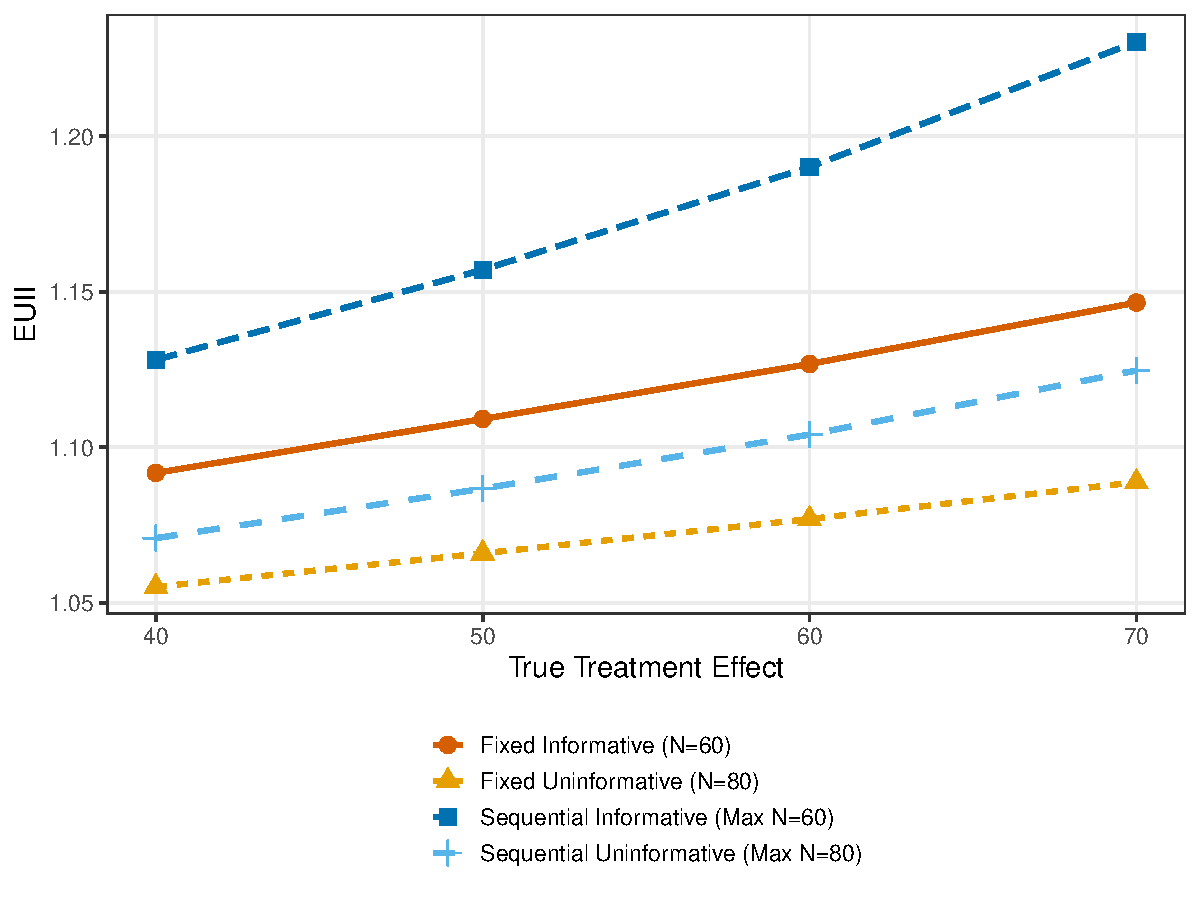
\includegraphics[width=\maxwidth]{figure/show-plot-1} 
\end{knitrout}
\caption{EUII Comparison}
\end{figure}

In Table \ref{sample_size_CRON} we can see the sample size for the two sequential designs:

% latex table generated in R 4.5.2 by xtable 1.8-8 package
% Thu Mar 19 13:25:09 2026
\begin{table}[ht]
\centering
\begin{tabular}{rrrrr}
  \toprule
$\Delta$ & $E[N_+]^{\text{info}}$ & $E[N_-]^{\text{info}}$ & $E[N_+]^{\text{uninfo}}$ & $E[N_-]^{\text{uninfo}}$ \\ 
  \midrule
40.00 & 35.66 & 41.73 & 45.37 & 57.60 \\ 
  50.00 & 35.55 & 41.44 & 45.84 & 57.38 \\ 
  60.00 & 34.62 & 41.13 & 45.67 & 57.11 \\ 
  70.00 & 33.25 & 40.90 & 44.76 & 56.88 \\ 
   \bottomrule
\end{tabular}
\caption{Sample size for sequential designs} 
\label{sample_size_CRON}
\end{table}


\textbf{NOTE}: in these plots and for the rest of the file, if not specified, the prior for the alternative used in the EUII computations is 10$\%$, i.e. $P(H_1) = 0.1$ 

\subsection{Sensitive analysis of varying the true value}
The idea here is to inspect what happens to the EUII when there is a mistake in specifyig the prior. \\
For this purpose, we fix the prior value for control: $\mu_{C, \text{prior}} = 49$, and we inspect the resulting EUII when the real control value ($\mu_{C, \text{true}}$) varies.
We define the prior bias:
$$b = \mu_{C, \text{true}} - \mu_{C, \text{prior}}$$ 
 
Note that we fix the true treatment effect $\Delta = 50$ and let $b$ vary. It's trivial to notice that the uninformative designs are not affected by varying $b$. 

The pattern is clear, as  $b$ increases from -20 to 20, both T1E and Power increases. Regarding the EUII, there is a slight decreasing trend, but the bumps are due to simulations. 
Infact, when $b<0$ (i.e. when $\alpha \approx 0$), the resulting EUII can vary. But in all seeds I tried, the decreasing trend was always present (not the bumps).
Brief intuitive explanation I thought of: \begin{itemize}
  \item Negative Bias ($b < 0$): The prior overestimates the true control mean. So the posterior estimate for the control is pushed higher than the data suggets.
  Since we don't have a prior on treatment, the resulting estimated treatment effect  ($\hat{\Delta} = \text{Treatment} - \text{Control}$) is reduced. Under $H_0$, 
  the model perceives the treatment as harmful, driving the Type-I Error ($\alpha$) to near zero. Under $H_1$, it becomes harder claim significance, so the Power reduces.
  \item Positive Bias ($b > 0$): The prior underestimates the true control mean. So the posterior estimate for the control group is pushed lower than reality. This inflates 
  the perceived treatment effect ($\hat{\Delta}$). Consequently, obtaining a significant result becomes much easier. This increases statistical Power, but also T1E.
\end{itemize}



\begin{figure}[h]
\centering
\begin{knitrout}
\definecolor{shadecolor}{rgb}{0.969, 0.969, 0.969}\color{fgcolor}
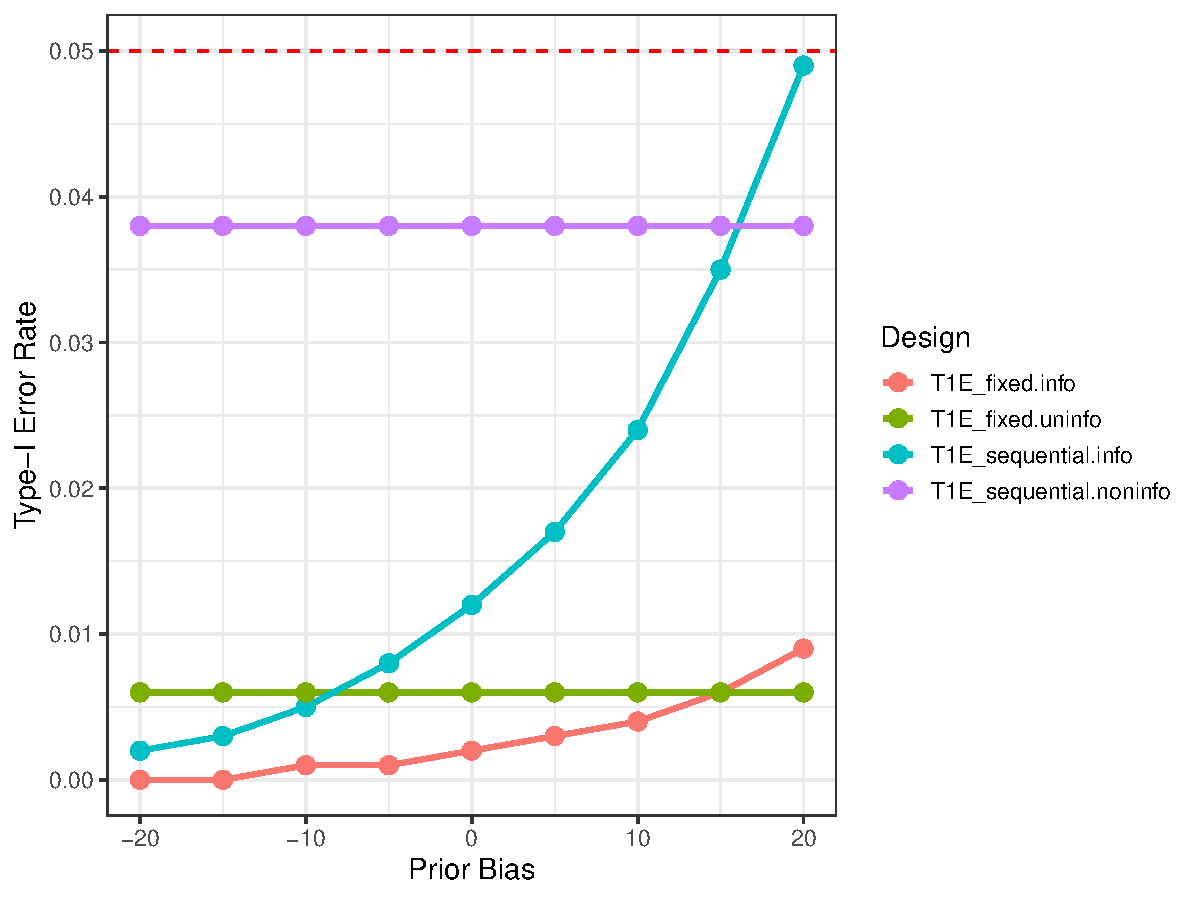
\includegraphics[width=\maxwidth]{figure/T1E_CRON-1} 
\end{knitrout}
\caption{T1E with varying prior bias}
\end{figure}



\begin{figure}[h]
\centering
\begin{knitrout}
\definecolor{shadecolor}{rgb}{0.969, 0.969, 0.969}\color{fgcolor}
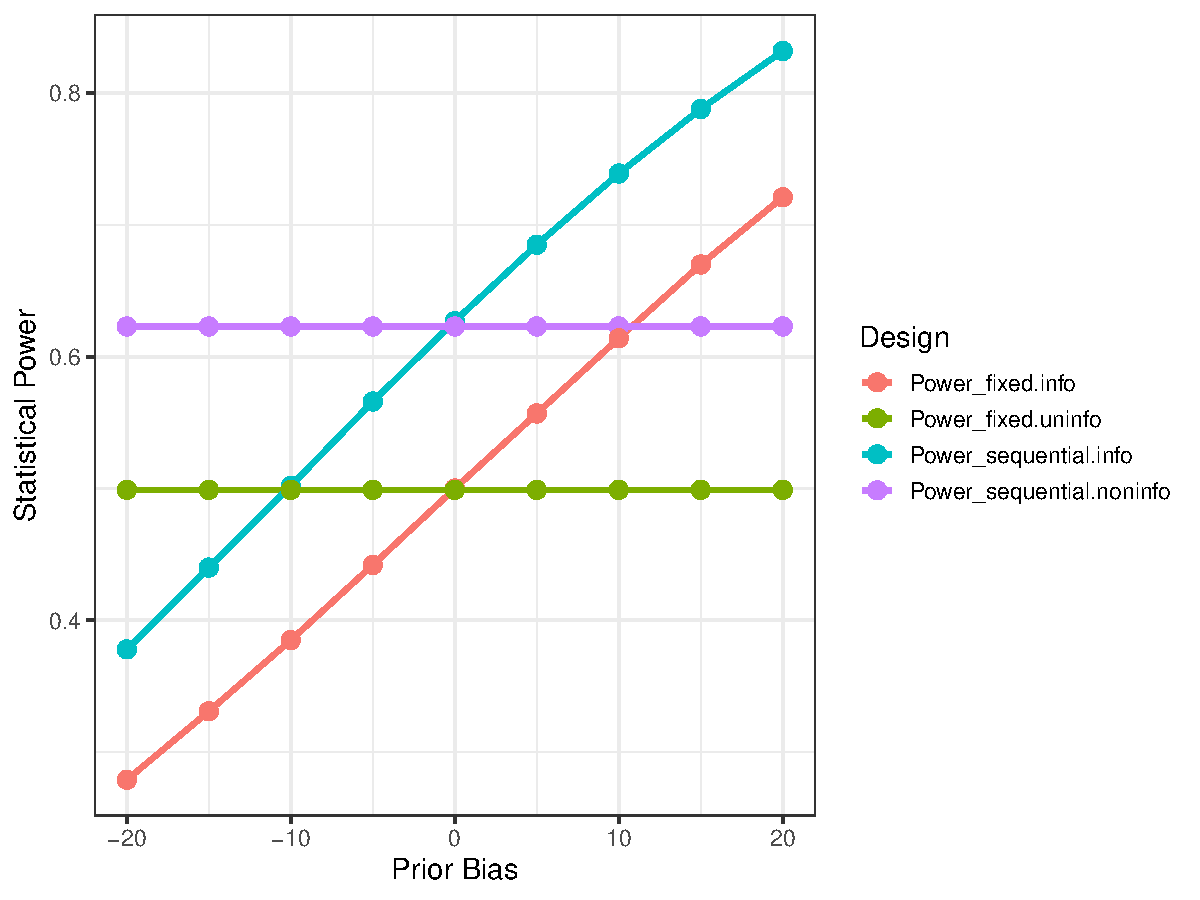
\includegraphics[width=\maxwidth]{figure/power_CRON-1} 
\end{knitrout}
\caption{Power with varying prior bias}
\end{figure}

\begin{figure}[h]
\centering
\begin{knitrout}
\definecolor{shadecolor}{rgb}{0.969, 0.969, 0.969}\color{fgcolor}
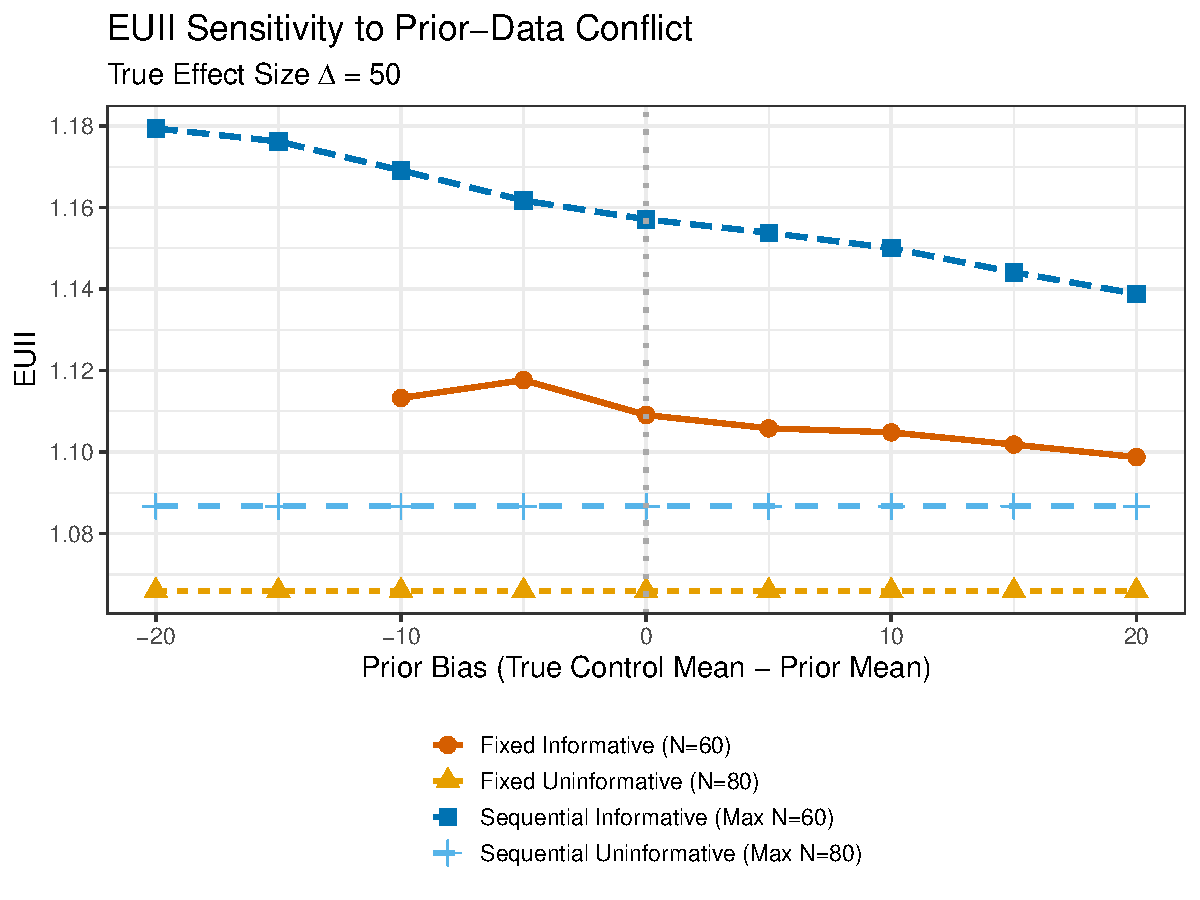
\includegraphics[width=\maxwidth]{figure/EUII_varying_delta_CRON-1} 
\end{knitrout}
\caption{EUII with varying prior bias}
\end{figure}

\FloatBarrier 





\section{Example 3.2: Oncology phase II single-arm trials}

This example in a single-arm oncology phase II trial where we have to decide if a new treatment has 
sufficient effect to invest in further development. Simon two-stage design is usually applied in
these cases. It is a \textit{two stage design} which allows for early stopping for futility but 
\textbf{No early stopping for success}. The design aims at minimizing the number of patients treated
with a drug with low activity. \\
To implement it in \texttt{gsbDesign}, we need normal approximation. It is well known that for binary data, the normal approximation is more appropriate
on the logit scale. Let $r_{Ei}$ be the number of responses and $n_{Ei}$ the number of treated patients in stage $i$, $i=c,E$. If we denote $y_{Ei}$ the 
log-odds of the observed response rate, its distribution is approximately: $$y_{Ei} \sim N(\text{logit}(\pi_E), \sigma_E^2/n_{Ei})$$
where $\pi_E$ is the underlying true response rate and $\sigma_E^2 = 1/(\pi_E) + 1/(1-\pi_E))$.\\

We need to mimic Simon's two-stage design, so we introduce a virtual control arm with no patients, $n_c$ with an extremely informative prior for 
$\pi_c$  (prior cenetered at the treu value with zero variance). \\
We set $\pi^*_c=0.4$, $\pi^*_E=0.6$, $\alpha=0.05$, and $\beta=0.20$. According to Simon's optimal two stage design, $n_{E1}=16$ patients are recruited 
in the first stage and $n_{E2}=30$ in the second stage. The trial is stopped for futility at the interim analysis if seven or less patients respond. 
The trial is a success at the end of the trial if more than 23 patients respond. Translating these criteria to the log-odds scale, the futility criterion 
is $$p(\delta < \text{logit}(7.5/16) - \text{logit}(0.4) \mid \text{Data}) \ge 0.5$$ and the success criterion is 
$$p(\delta > \text{logit}(23.5/46) - \text{logit}(0.4) \mid \text{Data}) \ge 0.5$$where $\delta = \text{logit}(\pi_E) - \text{logit}(\pi_C)$.
 
  
Note that early stopping for success is not allowed, this mean that $\E{N_+} = 46$ always. 

\subsection{Results}

% latex table generated in R 4.5.2 by xtable 1.8-8 package
% Thu Mar 19 13:25:10 2026
\begin{table}[ht]
\centering
\caption{Expected Total Sample Sizes (E[N]) for the Simon Two-Stage Optimal Design.} 
\label{tab:expected_N_onco}
\begin{tabular}{rrrrr}
  \toprule
control & treatment & delta & stage1 & stage2 \\ 
  \midrule
0.40 & 0.40 & 0.00 & 16.00 & 24.70 \\ 
  0.40 & 0.45 & 0.05 & 16.00 & 29.23 \\ 
  0.40 & 0.50 & 0.10 & 16.00 & 33.92 \\ 
  0.40 & 0.55 & 0.15 & 16.00 & 38.21 \\ 
  0.40 & 0.60 & 0.20 & 16.00 & 41.57 \\ 
   \bottomrule
\end{tabular}
\end{table}



% latex table generated in R 4.5.2 by xtable 1.8-8 package
% Thu Mar 19 13:25:10 2026
\begin{table}[ht]
\centering
\caption{EUII and other operating characteristics} 
\label{tab:comp_euii_onco}
\begin{tabular}{rrrrr}
  \toprule
True Rate delta ($\pi_E - \pi_C$) & DOR & EUII & $E[N_+]$ & $E[N_-]$ \\ 
  \midrule
0.05 & 3.60 & 1.0321 & 46.0 & 23.8 \\ 
  0.10 & 10.42 & 1.0648 & 46.0 & 23.8 \\ 
  0.15 & 27.22 & 1.1025 & 46.0 & 23.7 \\ 
  0.20 & 70.85 & 1.1490 & 46.0 & 23.6 \\ 
   \bottomrule
\end{tabular}
\end{table}





\begin{knitrout}
\definecolor{shadecolor}{rgb}{0.969, 0.969, 0.969}\color{fgcolor}\begin{figure}[h]

{\centering 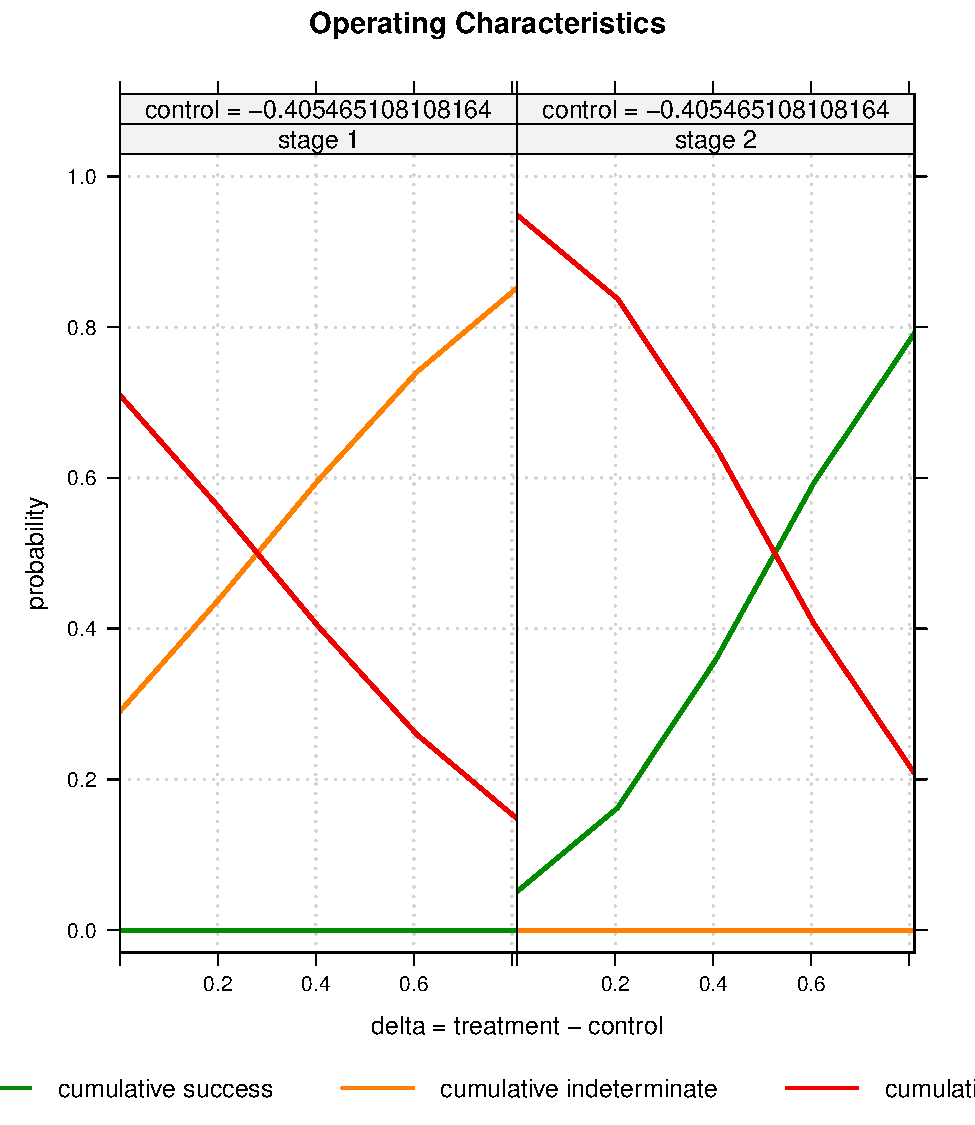
\includegraphics[width=\maxwidth]{figure/plot_OC_onco-1} 

}

\caption[Operating Characteristics]{Operating Characteristics.}\label{fig:plot_OC_onco}
\end{figure}

\end{knitrout}
 
Interestingly, the value of the prior for the alternative, doesnt have much influence here.
\begin{knitrout}
\definecolor{shadecolor}{rgb}{0.969, 0.969, 0.969}\color{fgcolor}\begin{figure}[h]

{\centering 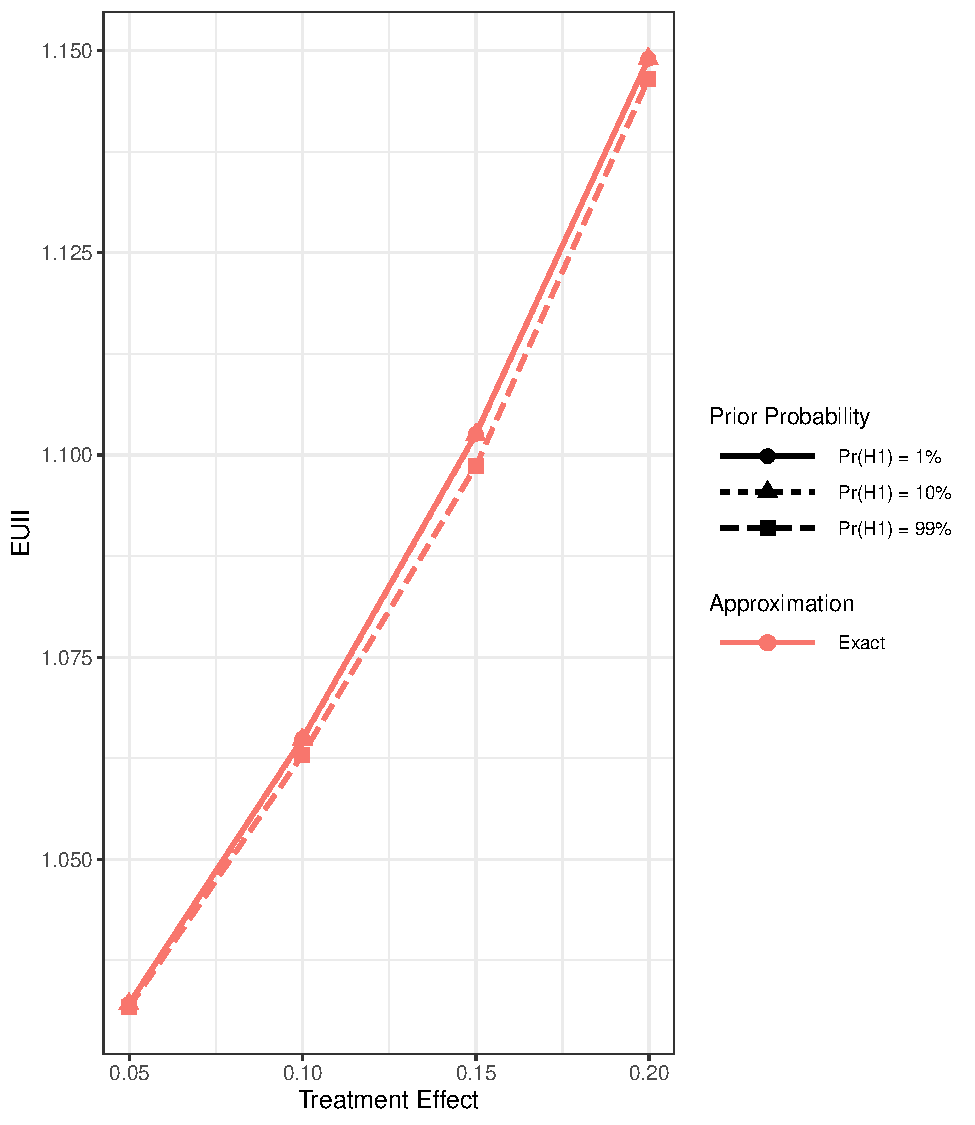
\includegraphics[width=\maxwidth]{figure/plot_EUII_onco-1} 

}

\caption[EUII with varying priors]{EUII with varying priors}\label{fig:plot_EUII_onco}
\end{figure}

\end{knitrout}



\FloatBarrier 

\section{Example 3.3. Design of a phase II trial in multiple sclerosis with
count endpoint}

In this example, the endpoint is MRI lesions \textbf{count}. The authors propose a Negative Binomial regression to model the count. 
Tipically, this model is fit using a log link function. 
We call $\kappa$ the assumed common over-dispersion paramete and $\mu_c$ and $\mu_E$ the underlying true mean MRI counts for control and experimental unit groups. Then, using the 
estimates $r_c$ and $r_E$. We can write the normal approximation as: 
$$  log(r_j) \sim N(\log(\mu_j), 1/\mu_j n_j + \kappa/n_j)$$
So we can define $\sigma_j^2 = 1/\mu_j + \kappa$.
This comes from the use of delta method following the parameterization of a negative binomial distribution given by \cite{Neg_Bin}:
\[
f(y) = \frac{\Gamma(y + 1/k) (\kappa \mu)^y} {\Gamma(y + 1) \Gamma(1/k) (1+\kappa \mu)^{y+1/k}} \quad \text{for } y = 0, 1, 2, \dots
\] 

\[
	\text{Dispersion} = \kappa \quad \Var{y} = \mu + \kappa \mu^2 \quad \E{y} = \mu
\] 


\begin{boxedproof}[Variance computation with Delta Method]
  
We know the delta method approximates the variance of a function of a random variable as:
\[
\mathrm{Var}\bigl[g(\hat{\theta})\bigr] \approx \bigl[g'(\theta)\bigr]^2 \Var{\hat{\theta}}
\]

For the log transformation $g(\mu) = \log(\mu)$ where $g'(\mu) = 1/\mu$:
\[
\mathrm{Var}\bigl[\log(\hat{\mu})\bigr] \approx \frac{\Var{\hat{\mu}}}{\mu^2}
\]

Using the negative binomial variance $\Var{\hat{\mu}} = \mu + \kappa \mu^2$:
\[
\mathrm{Var}\bigl[\log(\hat{\mu})\bigr] \approx \frac{\mu + \kappa \mu^2}{\mu^2} = \frac{1}{\mu} + \kappa 
\] 
\end{boxedproof}

Note that the variance of the log rate depends both on the mean $\mu$ and the over-dispersion parameter $\kappa$. \\

The design is a two-arms with 100 total subjects randomized with a 1:1 ratio and the interim analysis is planned
when final outcome is observed for $50\%$ patients, this mean that the interim analysis is planned when 25 patients per arm have completed the study.\\
Following Gsponer\cite{gsponer2014bayesian}, we fix $\kappa = 2$ and $\mu_c = 14.8$. \\
Denote $\delta = \log (\mu_c / \mu_E)$, to stop for early success, the following double criterion must be met: 
\[
P(\delta > 0 \mid \mathrm{Data}) > 0.9
\quad\text{and}\quad
P\!\left(\delta > \log(2.5)\mid \mathrm{Data}\right) > 0.5.
\]

This is equivalent to having a posterior median for \(\delta\) corresponding to at least a \(60\%\) relative reduction, with a \(90\%\) posterior probability of some reduction.

Whereas, in the case of stopping early for futility, a recommendation to stop would be based on the following double criterion:
\[
P\!\left(\delta < \log(1.43)\mid \mathrm{Data}\right) > 0.5
\quad\text{and}\quad
P\!\left(\delta < \log(2.5)\mid \mathrm{Data}\right) > 0.9.
\]
 
This rule is equivalent to having a posterior median for \(\delta\) corresponding to a risk reduction of less than \(30\%\), and a \(90\%\) posterior probability of \(\delta\) having a risk reduction of less than \(60\%\).\\

Additionally, an enthusiastic prior is obtained from Phase II trial, and it is not placed on the placebo, like the previous design, but \textbf{on the treatment effect} $\delta$. 
They observed a risk reduction of $75\%$ (i.e. $\delta = log(100/25) = log(4) $) in a trial consisting of 80 patients per group, with placebo rate and over-dispersion parameter equal
to the planning assumptions stated previously.This prior is considered to be worth 10 patients per grpup.\\

\subsection{Results}
Table \ref{tab:expected_N} illustrates the Expected Total Sample Size ($E[N]$) across varying true treatment effects for both the Non-Informative and Informative. Since the trial needs at least 50 patients, 
values close to 50 indicate a high probability of early stopping, while values close to 100 indicates that the trial frequently required both stages to reach a decision.

Intuitively, when the true treatment effect is close to the prior's value (e.g., $75\%$ relative reduction), the Informative design proves to require less patients.

However, if the drug underperforms with respect to the prior, the sample size of the informative increases. At a 0\% relative reduction (the null hypothesis), the Non-Informative design identifies futility efficiently, 
stopping the trial at an expected 59.1 patients. In contrast, the Informative design requires an expected 75.8 patients.

% latex table generated in R 4.5.2 by xtable 1.8-8 package
% Thu Mar 19 13:25:10 2026
\begin{table}[ht]
\centering
\caption{Comparison of Expected Total Sample Sizes (E[N]) under Non-Informative and Informative Priors.} 
\label{tab:expected_N}
\begin{tabular}{rrr}
  \toprule
True Reduction (\%) & E[N] Non-Informative & E[N] Informative \\ 
  \midrule
0 & 58.9 & 75.8 \\ 
  5 & 60.4 & 77.7 \\ 
  10 & 62.2 & 79.5 \\ 
  15 & 64.2 & 81.0 \\ 
  20 & 66.3 & 82.2 \\ 
  25 & 68.5 & 82.9 \\ 
  30 & 70.7 & 83.1 \\ 
  35 & 72.7 & 82.5 \\ 
  40 & 74.3 & 80.9 \\ 
  45 & 75.1 & 78.5 \\ 
  50 & 75.0 & 75.0 \\ 
  55 & 73.6 & 70.7 \\ 
  60 & 70.6 & 65.7 \\ 
  65 & 66.3 & 60.7 \\ 
  70 & 61.2 & 56.2 \\ 
  75 & 56.1 & 52.8 \\ 
  80 & 52.4 & 50.9 \\ 
  85 & 50.5 & 50.1 \\ 
  90 & 50.0 & 50.0 \\ 
   \bottomrule
\end{tabular}
\end{table}



Figure \ref{fig:euii_dashboard} shows that the EUII is strictly larger for the Non-Informative design across every signle scenario.
The reason can be come from that while the informative prior saves about 3 to 4 patients when correctly rejecting $H_0$, it costs many patients when failing to reject it. This mean that the EUII 
is dragged down.

Another reason can be that having the entusiastic prior leads to an increased Power for some alternatives, but also increased T1E. This can in turn lead to a reduced DOR. 

Note, when the true reduction is $85 \%$ and $90 \%$, $ P(-) = 0$, this mean that it is impossible to compute the EUII since the trial always ends up in a success. 



\begin{knitrout}
\definecolor{shadecolor}{rgb}{0.969, 0.969, 0.969}\color{fgcolor}\begin{figure}[h]

{\centering 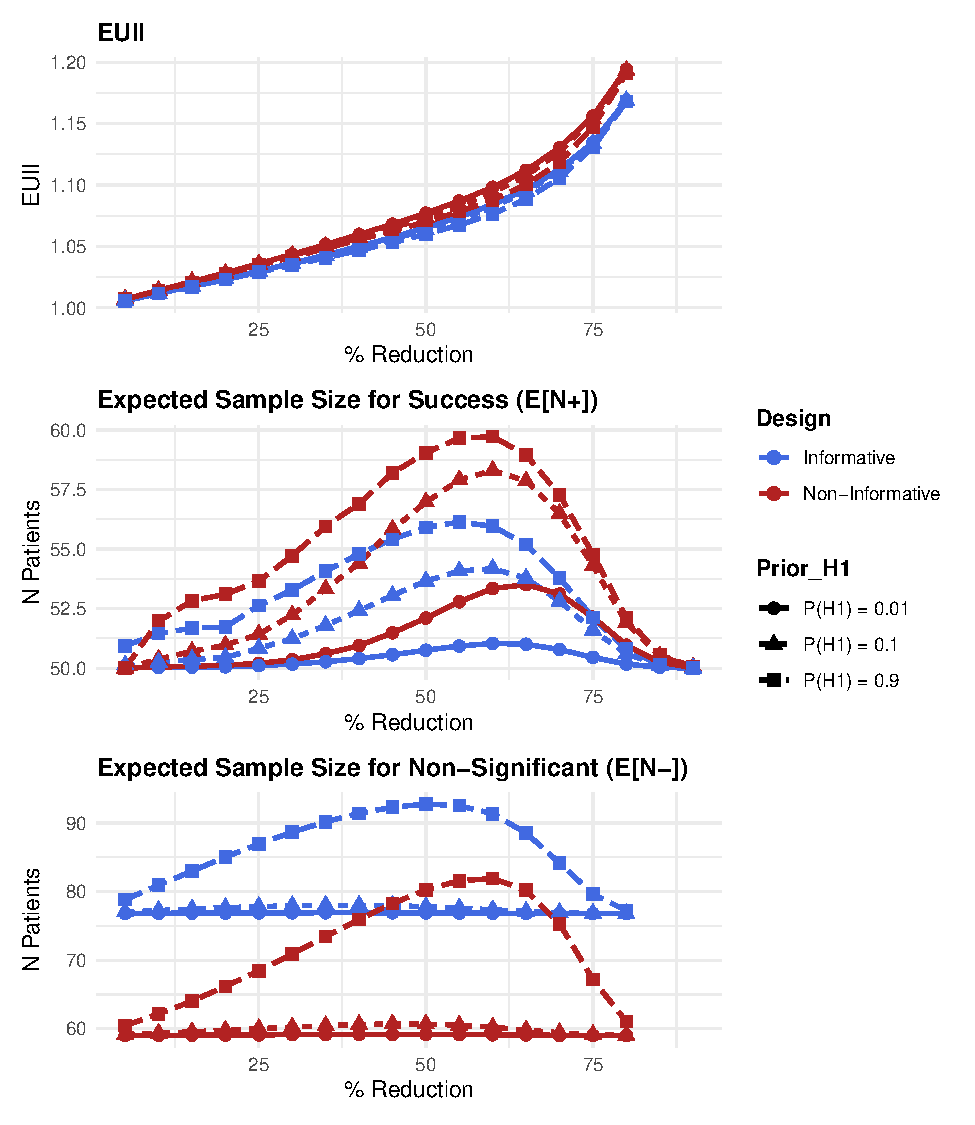
\includegraphics[width=\maxwidth]{figure/plot_dashboard-1} 

}

\caption{EUII under varying priors.\label{fig:euii_dashboard}}\label{fig:plot_dashboard}
\end{figure}

\end{knitrout}



% latex table generated in R 4.5.2 by xtable 1.8-8 package
% Thu Mar 19 13:25:12 2026
\begin{table}[ht]
\centering
\caption{Comparison of EUII and Conditional Expected Sample Sizes between informative and non informative} 
\label{tab:comp_euii}
\begin{tabular}{rrrrrrr}
  \toprule
True Red. (\%) & EUII (Non-Inf) & EUII (Inf) & $E[N_+]$ (Non-Inf) & $E[N_+]$ (Inf) & $E[N_-]$ (Non-Inf) & $E[N_-]$ (Inf) \\ 
  \midrule
5 & 1.0071 & 1.0058 & 50.0 & 50.1 & 59.2 & 77.0 \\ 
  10 & 1.0141 & 1.0117 & 50.4 & 50.3 & 59.4 & 77.2 \\ 
  15 & 1.0213 & 1.0175 & 50.7 & 50.4 & 59.6 & 77.5 \\ 
  20 & 1.0281 & 1.0235 & 51.0 & 50.4 & 59.8 & 77.7 \\ 
  25 & 1.0356 & 1.0297 & 51.4 & 50.8 & 60.0 & 77.8 \\ 
  30 & 1.0427 & 1.0359 & 52.2 & 51.2 & 60.2 & 77.9 \\ 
  35 & 1.0501 & 1.0424 & 53.3 & 51.8 & 60.5 & 78.0 \\ 
  40 & 1.0576 & 1.0490 & 54.4 & 52.4 & 60.6 & 78.0 \\ 
  45 & 1.0652 & 1.0560 & 55.8 & 53.1 & 60.7 & 77.9 \\ 
  50 & 1.0734 & 1.0635 & 57.0 & 53.7 & 60.7 & 77.8 \\ 
  55 & 1.0827 & 1.0720 & 57.9 & 54.1 & 60.5 & 77.6 \\ 
  60 & 1.0937 & 1.0820 & 58.3 & 54.2 & 60.2 & 77.3 \\ 
  65 & 1.1078 & 1.0946 & 57.9 & 53.8 & 59.8 & 77.1 \\ 
  70 & 1.1268 & 1.1112 & 56.5 & 52.8 & 59.4 & 76.9 \\ 
  75 & 1.1539 & 1.1337 & 54.3 & 51.6 & 59.1 & 76.8 \\ 
  80 & 1.1933 & 1.1687 & 51.9 & 50.6 & 59.0 & 76.8 \\ 
  85 &  &  & 50.5 & 50.1 &  &  \\ 
  90 &  &  & 50.0 & 50.0 &  &  \\ 
   \bottomrule
\end{tabular}
\end{table}


\begin{knitrout}
\definecolor{shadecolor}{rgb}{0.969, 0.969, 0.969}\color{fgcolor}\begin{figure}[h]

{\centering 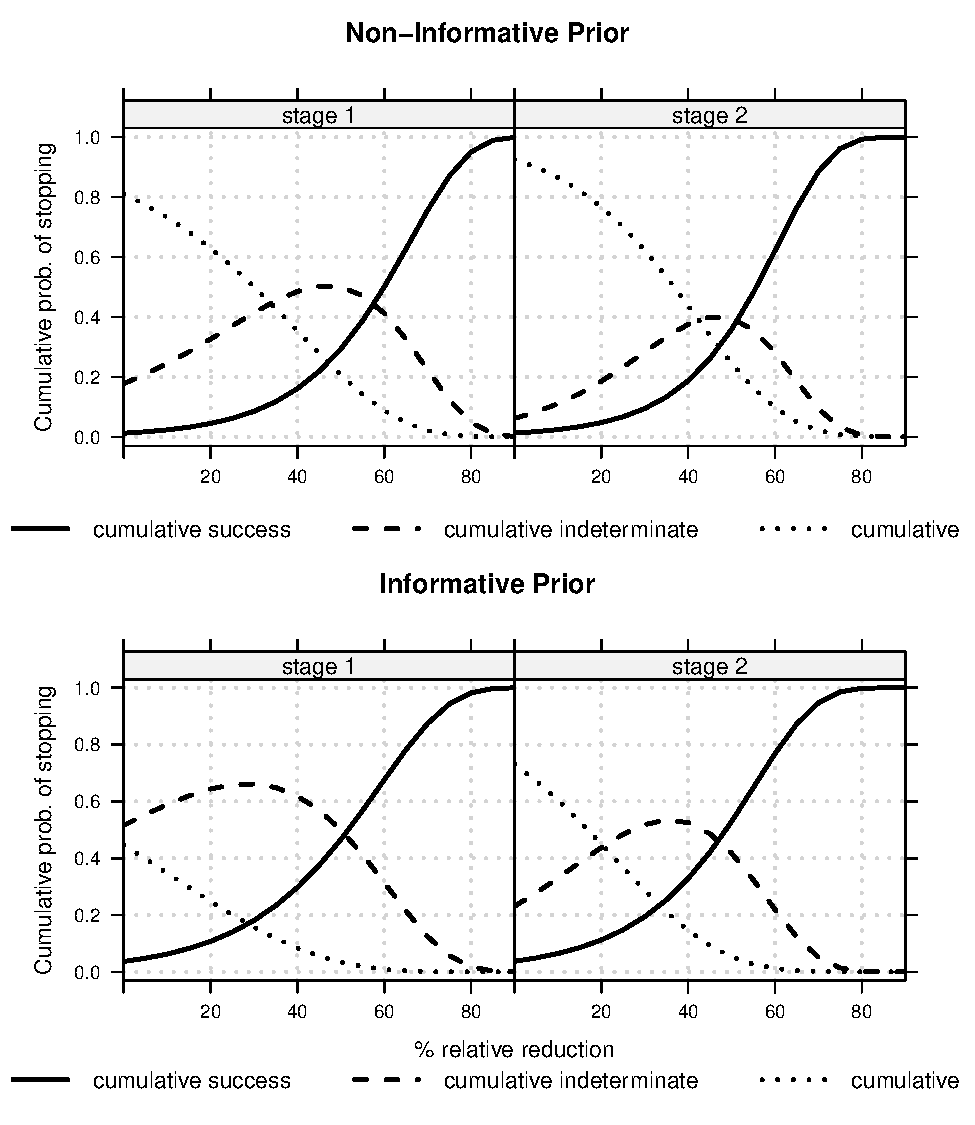
\includegraphics[width=\maxwidth]{figure/plot_oc-1} 

}

\caption[Cumulative probability of stopping for the Non-Informative and Informative prior designs]{Cumulative probability of stopping for the Non-Informative and Informative prior designs.}\label{fig:plot_oc}
\end{figure}

\end{knitrout}
 


\FloatBarrier 

\section{Example 3.4. A phase III trial design with Bayesian futility criteria for
a time-to-event endpoint}

In the context of survival analysis, the measure of treatment effect used is often Hazard Ratio. 

Let $\lambda_1(t)$ and $\lambda_0(t)$ be the hazard functions for the test and control groups, respectively.
Under the proportional hazards assumption, the hazard ratio is constant over time: $HR = \lambda_1(t) / \lambda_0(t)$.

We define the treatment effect $\theta = \log(HR)$ and we can use the standard asymptotic normal approximation for the estimate of the log hazard ratio 
under the assumption of equal survival distributions:
$$\hat{\theta} \sim N\left(\theta, \frac{c}{E_1 + E_2}\right)$$
for a k:1 randomization where $c = (k+1)^2 /k$ and $E_1$ $E_2$ are the events in test and control group. \\
For a 1:1 randomization, $c = 4$ $E_1 + E_2 = E$ and we can define: $$\text{Var}(\hat{\theta}) = \frac{4}{E}$$

Since gsbDesign computes the variance of $\hat{\delta}$ as $$\text{Var}(\hat{\delta}) = \frac{\sigma_E^2}{n_E} + \frac{\sigma_C^2}{n_C}$$
Setting $\sigma_T = 1$ and $\sigma_C = 1$,  $$Var(\hat{\delta}) = \frac{1^2}{E_{arm}} + \frac{1^2}{E_{arm}} = \frac{2}{E_{arm}}$$ Since the total number of events 
across both arms is $E_{total} = 2 \times E_{arm}$, we can substitute $E_{arm} = E_{total} / 2$: $$Var(\hat{\delta}) = \frac{2}{E_{total} / 2} = \frac{4}{E_{total}}$$.
So by setting \texttt{sigma = c(1,1)} in the paper we mapped the asymptotic vairance into the gsbDDesign.

For a more general case using hazard ratios, the authors suggest to use the formula $\sigma_1 = \sigma_2 = \sqrt{c E_1 E_2 / (E_1 + E_2)^2}$  to implement in the software. 
To represent positive values as beneficial treatment effect, we define the parameter $\delta = -\theta = \log(1/HR)$. Consequently, a hazard ratio less 
than 1 (indicating a reduction in the risk of an event) results in a positive value for $\delta$. The non-inferiority margin is defined as $HR_{NI} = 1.075$, 
which corresponds to $\delta_{NI} = -\log(1.075) \approx -0.0723$.\\

The design consists of three stages with interim analyses after $1/3$ and $2/3$ of the total expected events have occurred. Assuming $E_{total} = 1800$ events, 
each stage accrues 600 events. Under the null hypothesis of equal survival distributions ($E_1 = E_2$), this corresponds to 300 events per treatment group per stage. \\

The original trial used modified Haybittle Peto boundaries for stopping for success, requiring a high posterior probability of superiority at the interims 
($P(\delta > 0 | D) > 0.99995$ and $P(\delta > 0 | D) > 0.9995$) and a standard probability of non-inferiority at the final analysis ($P(\delta > \delta_{NI} | D) > 0.975$). \\

The final trial was a massive waste of money since it concluded withouth any evidence. The paper argue that adding bayesian futility stopping rules could have saved resources. 
Stage 1: Stop if $P(\delta < \delta_{NI} | D) > 0.95$ Stage 2: Stop if $P(\delta < \delta_{NI} | D) > 0.90$ Stage 3: Stop if $P(\delta < \delta_{NI} | D) > 0.80$

\subsection{Results}
\begin{center}
\resizebox{\textwidth}{!}{%
% latex table generated in R 4.5.2 by xtable 1.8-8 package
% Thu Mar 19 13:25:13 2026
\begin{tabular}{rrrrrrr}
  \toprule
True HR & EUII (Orig) & EUII (Bayes) & $E[Events_+]$ (Orig) & $E[Events_+]$ (Bayes) & $E[Events_-]$ (Orig) & $E[Events_-]$ (Bayes) \\ 
  \midrule
0.861 & 1.0056 & 1.0060 & 1669.394 & 1669.394 & 1786.466 & 1694.805 \\ 
  0.900 & 1.0040 & 1.0042 & 1761.648 & 1761.648 & 1786.517 & 1695.199 \\ 
  0.951 & 1.0026 & 1.0027 & 1794.387 & 1794.387 & 1786.855 & 1697.699 \\ 
  1.000 & 1.0017 & 1.0017 & 1798.929 & 1798.929 & 1787.352 & 1701.165 \\ 
  1.051 & 1.0006 & 1.0006 & 1800.000 & 1800.000 & 1787.204 & 1699.299 \\ 
  1.073 & 1.0001 & 1.0001 & 1800.000 & 1800.000 & 1786.580 & 1695.414 \\ 
  1.100 & 0.9993 & 0.9993 & 1800.000 & 1800.000 & 1784.521 & 1687.101 \\ 
  1.150 &  &  &  &  & 1774.957 & 1663.120 \\ 
   \bottomrule
\end{tabular}

}
\end{center}
 
Note the EUII smaller tha 1 when HR larger than 1.075 (since it is a noninferiority trial). This because if HR larger than 1, the drug is actually harmful. 
This lead to a $LR_+ < 1$, so $Power < T1E$ and as established by Lehmann (1959), a test where the power to reject the null is smaller than the TIE rate is formally called a "biased test".

This mean that DOR is smaller than 1, which in turn lead to a EUII smaller 1. \\
Recall that $DOR = O(H1|+) / O (H1|-)$, where $O(H1|+)$ is the odds of H1 being true given a significant result. If $DOR < 1$, then a significant result leaves you with lower odds of H1 being true than a non-significant result. 



\begin{knitrout}
\definecolor{shadecolor}{rgb}{0.969, 0.969, 0.969}\color{fgcolor}\begin{figure}[h]

{\centering 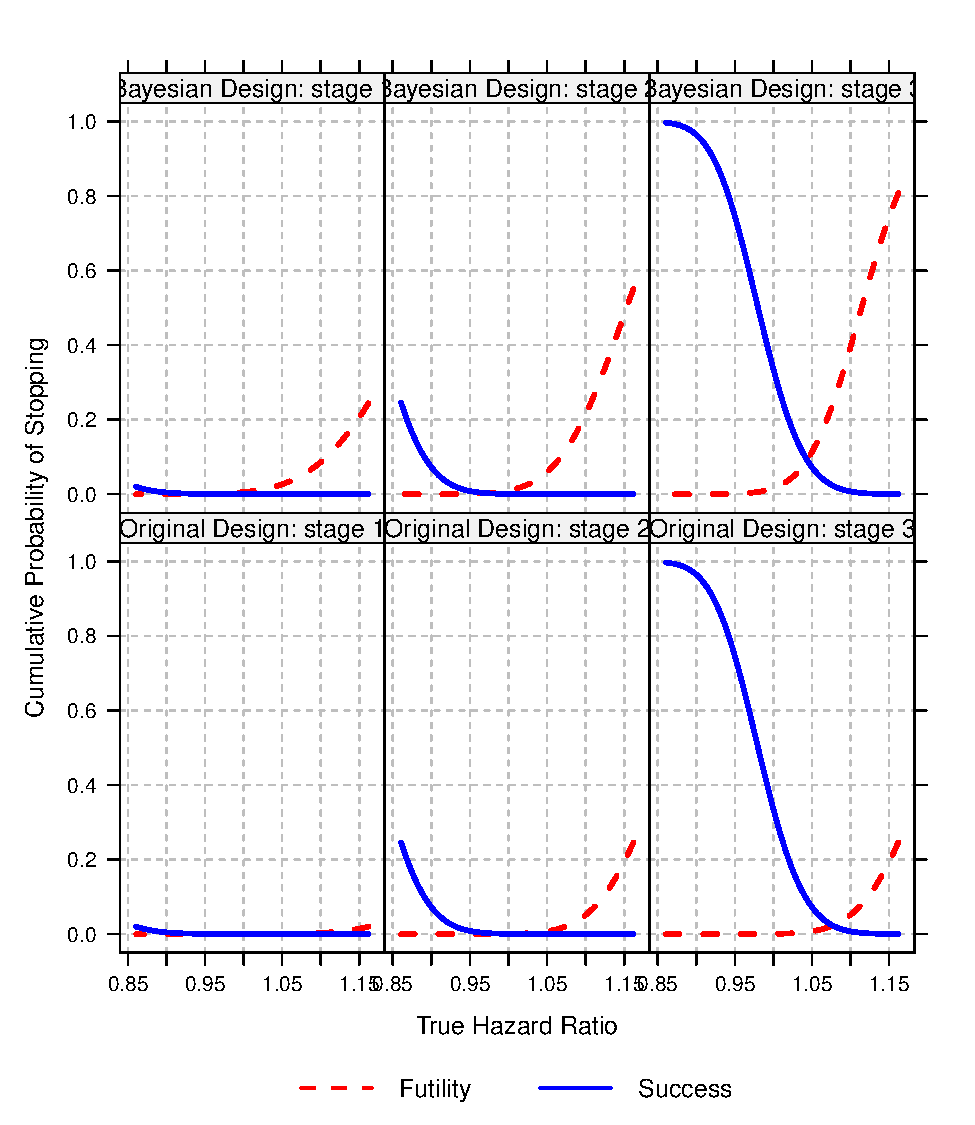
\includegraphics[width=\maxwidth]{figure/plot_1-1} 

}

\caption[Hazard Ratio]{Hazard Ratio}\label{fig:plot_1}
\end{figure}

\end{knitrout}

\begin{knitrout}
\definecolor{shadecolor}{rgb}{0.969, 0.969, 0.969}\color{fgcolor}\begin{figure}[h]

{\centering 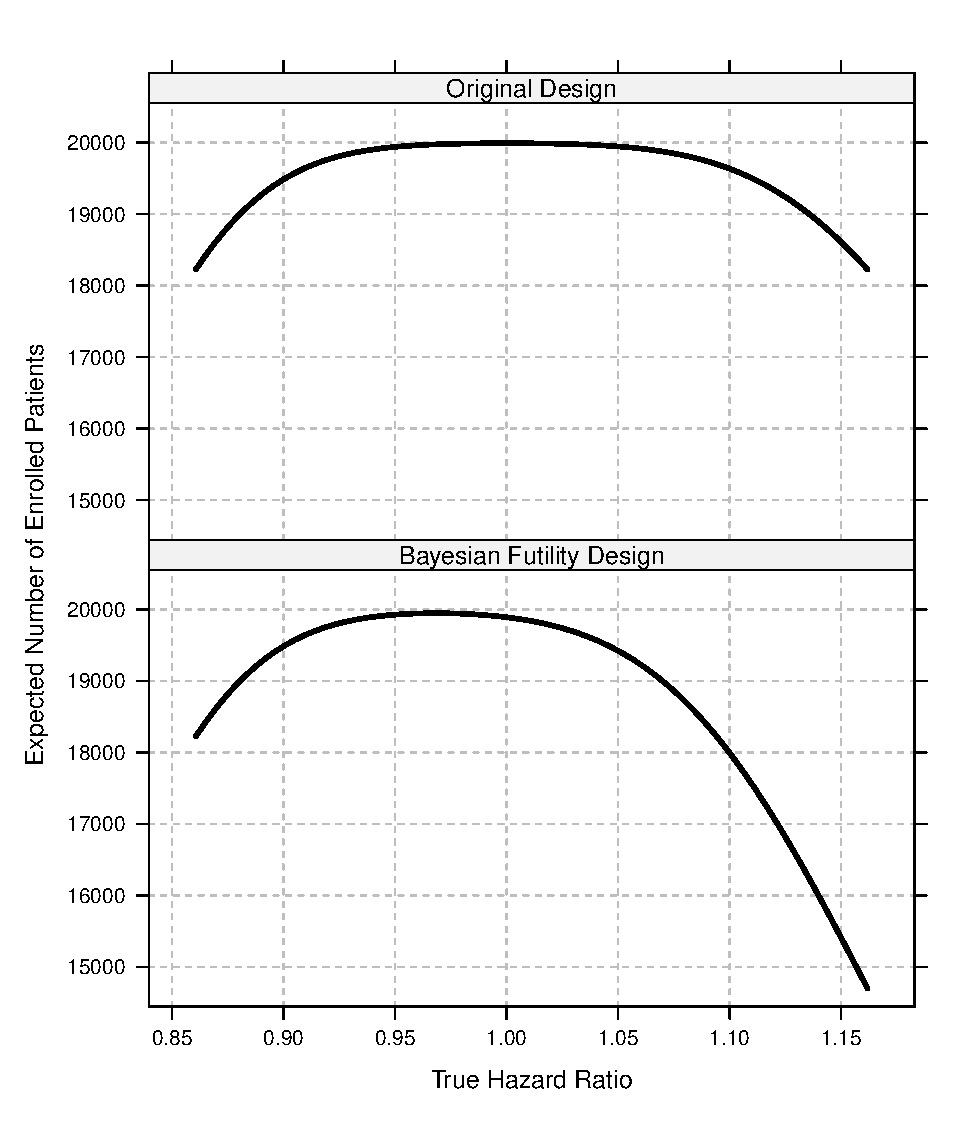
\includegraphics[width=\maxwidth]{figure/plot_2-1} 

}

\caption[Hazard Ratio]{Hazard Ratio}\label{fig:plot_2}
\end{figure}

\end{knitrout}

\FloatBarrier 
 
\newpage
\bibliography{references}   
\end{document}
  
 
    
